%% The Self-Compiling Learner
%% ACM sigconf draft. Build: pdflatex selfcompiler && bibtex selfcompiler && pdflatex x2
%% Figures: .venv/bin/python paper/selfcompiler/make_figures.py
%% Every number is a committed result; the provenance map is NUMBERS.md.
\documentclass[sigconf,nonacm]{acmart}

\settopmatter{printacmref=false}
\setcopyright{none}
\renewcommand\footnotetextcopyrightpermission[1]{}

\usepackage{booktabs}
\usepackage{amsmath}

\newcommand{\code}[1]{\texttt{#1}}
\newcommand{\tagp}[1]{\textsc{\small[#1]}}

\begin{document}

\title{The Self-Compiling Learner: Crystallizing Language-Model Behavior into
Certified, Served Rule Programs}

\author{J. Allan Scott}
\affiliation{\institution{}\country{}}

\begin{abstract}
We present a continual learner whose consolidation phase is a \emph{compiler}: during wake it
learns soft relational circuits by plain SGD; during sleep it hardens them to discreteness,
extracts their programs mechanically from the weights, certifies the extractions with an exact
Datalog engine, installs the certified rules as gradient-free structure, and returns the freed
capacity to the pool. A certified rule is forgetting-proof because it is no longer weights. On a
synthetic curriculum the compile arm retains all tasks perfectly ($1.000/1.000/1.000$) where a
matched-budget baseline collapses ($0.010/0.002/0.007$); the flagship circuit --- a discrete
induction head learned by plain SGD --- carries a machine-checked certificate of exact agreement
with a three-line Datalog program on its full test domain (2048/2048). Pointed at real text and at
the Pythia model family as teachers, the learner's judge admits exact rules only when they pay on
held-out data, and the resulting \emph{certified core} --- a count table plus a handful of proved
rules, served host-side with citations and honest abstention --- captures a fraction of teacher
behavior that does \emph{not} collapse with teacher scale (crystallization rises to a
$\sim$85\% plateau across $200\times$ parameters) and, under support-weighted arbitration, can
\emph{exceed the student that discovered the rules} (0.60 vs.\ 0.57 agreement with a code-domain
teacher). An independent corpus-statistics decompiler agrees with the learned rules on 99.2\% of
the contexts both cover, giving two-instrument confirmation of what the teacher is. We report
methodology as first-class results: every claim carries a proved/empirical tag over a stated
domain, and the paper's negative results --- a conjunction-free benchmark, admission by
val-variance noise, a cover-order bottleneck worth more than every rule family combined --- were
each caught by the machinery itself.
\end{abstract}

\maketitle

\section{Introduction}

Two research programs approach the same artifact from opposite sides. \emph{Mechanistic
interpretability} starts from a trained transformer and mines circuits out of frozen weights;
\emph{neurosymbolic learning} starts from symbols and asks how much behavior rules can carry.
This paper builds the bridge as a single running system: a learner that behaves like a small
language model while it runs, and like a decompiler while it sleeps.

The system rests on three design commitments. First, \textbf{memorization is structural}: a
lookup table updated by counting, not by gradient --- plain SGD provably underfits lookup tables,
and a count table is what our serving format ships anyway. Second, \textbf{relational computation
is a rule form}: a relational head is a T3 threshold gate $\times$ a bilinear matcher over raw
token codes $\times$ \emph{successor routing} (copy what followed the matched position), with a
decode tied to the token-code table. This is an attention head restated as a discrete gather, and
it is the form that makes extraction possible. Third, \textbf{consolidation is compilation}: sleep
does not merely protect weights (cf.\ EWC~\cite{kirkpatrick2017ewc}); it anneals a circuit to its
hard-routed self, reads the program out of the weights, certifies the program against the
circuit's own behavior with Souffl\'e~\cite{jouppi2016souffle}, and replaces the circuit with the
program.

\textbf{Contributions.}
\begin{enumerate}
\item A relational rule head that learns the canonical attention circuit (induction) to
$0.999$ accuracy under \emph{plain SGD}, hard-routes at $0.998$, and --- after a hardening anneal
--- carries a certificate of exact agreement with a three-line Datalog program on all 2048 test
windows \tagp{proved, stated domain}. The extraction is mechanical: family from the vocabulary
match matrix, guards from the certified data domain, tie-breaks from the architectural form
(\S\ref{sec:circuits}).
\item \textbf{Sleep-as-compilation}: a wake/sleep~\cite{hintonwakesleep1995} loop in which
certified rules are installed as preempting structure and their soft sources are recycled.
Zero forgetting on a three-task curriculum without replay, against a matched-budget baseline that
forgets everything (\S\ref{sec:compile}); the same loop, run autonomously on real text, discovers
and installs its rules by a held-out admission judge and \emph{beats the hand-built variant}
(\S\ref{sec:text}).
\item \textbf{The certifiability scaling law}: across the Pythia ladder
(14M--2.8B)~\cite{biderman2023pythia}, the certified fraction of teacher behavior declines only
gently ($0.285\!\to\!0.230$, near-flat above 410M) while the \emph{crystallization ratio} ---
certified core over student --- rises from 74\% to a $\sim$85\% plateau (\S\ref{sec:scaling}).
\item \textbf{The race}: the learning route and an independent corpus-statistics decompiler,
pointed at the same teacher on the same data, agree on \textbf{99.2\%} of the contexts both
cover --- two instruments confirming each other --- while optimizing opposite operating points
(total imitation vs.\ precision-with-abstention) (\S\ref{sec:race}).
\item A rule-library study whose sharpest finding is architectural: with a fixed-priority cover,
added rule families mostly \emph{displace} the count tier; replacing priority with
\textbf{support-weighted arbitration} (Laplace-shrunk per-key determinism; one confidence field
for scalar kinds) is worth more than every family combined --- it doubles the certified core on
code, where the core then \emph{exceeds the soft student that discovered the rules}
(\S\ref{sec:library}).
\item A deployment path: a \code{relation} schema kind (eq-guard + copy) landed across the
package schema and two runtimes with verified parity, and per-dataset experts federated under an
abstention-routing hub, every answer citing the sleep cycle that admitted its rule
(\S\ref{sec:deploy}).
\end{enumerate}

\textbf{Methodology as a result.} Every claim below carries a tag --- \tagp{proved} only with a
machine-checked artifact over a stated domain, otherwise \tagp{empirical} --- and the paper's
corrections were produced by its own machinery: an exact certificate caught a mirror bug; a
val-variance analysis caught noise admissions; the reference number the project inherited
($0.189$ ``teacher decode'') was itself exposed as a probe artifact (the true value is $0.244$).
A full provenance map from every table to its commit and log ships with the paper
(\code{NUMBERS.md}).

\section{Related Work}

\textbf{Induction heads and circuits.} The induction head is the best-understood transformer
circuit~\cite{elhage2021framework,olsson2022induction}; we learn it as a discrete rule, certify
it exactly, and measure its durability across scale (the teacher-side copy-pattern incidence
declines only from 28\% to 23.5\% over 200$\times$ parameters, and is 66--69\% on code).
\textbf{Rule induction.} Our proposers are deliberately classical: sequential covering and
conditional refinement (CN2~\cite{clark1989cn2}, FOIL~\cite{quinlan1990foil},
RIPPER~\cite{cohen1995ripper}, ILP~\cite{muggleton1991ilp}) reappear as interaction-scored,
error-driven frame mining; the negative result that \emph{marginal} scoring cannot beat a linear
path is a corollary the field knew. \textbf{Wake/sleep and library learning.} The loop is
wake/sleep~\cite{hintonwakesleep1995} with DreamCoder's library-growth
instinct~\cite{ellis2021dreamcoder}, but the consolidation product is a \emph{certificate}, not a
posterior. \textbf{Distillation.} Teacher imitation~\cite{hinton2015distilling} here targets
\emph{decisions} and asks a different question: not how small a student can be, but how much of
the teacher crystallizes into exact structure. \textbf{Model decompilation.} The comparison
decompiler (the analysis route of \S\ref{sec:race}) mines gated $n$-grams and causal idioms from
corpus statistics and frozen weights; the two routes' 99.2\% agreement where they overlap is, to
our knowledge, the first two-instrument cross-validation of a decompiled artifact.

\section{The Learner}
\label{sec:learner}

\textbf{Substrate.} Token codes $C \in \mathbb{R}^{V\times K}$ are \emph{frozen} after
initialization from a teacher's embedding geometry (PCA, z-scored) --- grounding buys the linear
path $+0.023$ agreement and, decisively, gives continual learning a stationary concept space: with
a trainable $C$ and a tied decode, training task $k$ back-propagates into every class row and
wrecks unseen tasks \tagp{empirical}.

\textbf{Paths.} (i) a \emph{count tier}: an online table over the stream (bigram; later $k$-gram
tiers with the same online semantics); (ii) a \emph{relational head}: T3 gate
$\sigma(\beta(\rho^\top \ell - \theta))$ over query literals, bilinear matcher
$s_i = \phi_i^\top A\, q/\sqrt{K} + u^\top \phi_i$ over raw position codes $\phi_i$ (near-orthogonality
is what the matcher needs; sigmoid-squashed features sit at chance), softmax routing over
positions, and \emph{successor routing}: the value written back is the matched position's
successor code; decode is tied, $\mathrm{logits} = qC^\top$; (iii) \emph{installed rules}: exact
programs that preempt (\S\ref{sec:compile}).

\textbf{Wake/sleep.} Wake trains continuous parameters with plain SGD over a streaming episode
and updates count tiers. Sleep is structural: harden, extract, certify, install, recycle
(\S\ref{sec:compile}); propose and judge library candidates (\S\ref{sec:library}). Sleep may use
heavier optimization (Adam, annealing) --- consolidation is not the wake learner.

\textbf{The judge.} A rule is admitted only if it improves held-out validation agreement ---
measured \emph{under the same cover semantics the runtime will realize}
(\S\ref{sec:library}) --- beyond a threshold; high-variance families carry stricter thresholds.

\section{Certified Relational Circuits}
\label{sec:circuits}

We test the head where attention's work is the ground truth: \emph{induction}
($\dots A\,B \dots A \to B$, context 128), \emph{marker} (predict the successor of a unique
marker token), and \emph{khop2} (two chained lookups through a bridge token).

\begin{table}[h]
\caption{The battery (L=128; every baseline lr-piloted; the transformer receives $\sim$4$\times$
the student's steps). Hard-route = one-hot routing at evaluation. \tagp{empirical} except where
noted.}
\label{tab:battery}
\small
\begin{tabular}{lcccc}
\toprule
task & old form & transformer 2L (30k) & \textbf{head (SGD)} & hard-route \\
\midrule
induction & 0.022 & 0.023 & \textbf{0.999} & \textbf{0.998} \\
marker & 0.019 & 1.000 & \textbf{1.000} & \textbf{1.000} \\
khop2 & 0.008 & 0.005 & 0.010 & --- \\
khop2 (Adam) & & & 0.920 & 0.224 \\
\bottomrule
\end{tabular}
\end{table}

The transformer is not a strawman --- it reaches $1.000$ on marker; it simply never undergoes the
induction phase transition at this scale and budget, while the rule form has the circuit's shape
built in, so gradient only has to find the matcher.

\textbf{Hardening to proved.} A temperature anneal ($\beta{:}\,1\!\to\!24$) with a
straight-through finish takes induction to soft $=$ hard $= 1.000$, and the certificate ---
tensor hard-route vs.\ the Datalog program
$\mathit{hit}(w,p) \leftarrow \mathit{tok}(w,p,t), \mathit{qtok}(w,t)$;
$\mathit{best} = \max \mathit{hit}$; $\mathit{pred} = \mathit{successor}(\mathit{best})$ ---
reaches \textbf{2048/2048} \tagp{proved, on the stated 2048-window domain}. The same anneal makes
khop2 \emph{discrete} ($0.987 = 0.987$), closing the multi-hop softness wall (with Adam in sleep;
wake-SGD-only multi-hop remains open).

\textbf{Mechanical extraction.} Scanning all (layer, head) pairs for fidelity, checking the
vocabulary match matrix $M(a,b)=\phi_a^\top A\, C_b$ for diagonal dominance (token equality),
checking gate saturation, and reading successor routing and most-recent tie-break from the form,
the program is \emph{assembled from findings} and verified extensionally: extracted $\equiv$
hand-written $\equiv$ tensor on all 2048 windows. The exactness matters: the Souffl\'e check
caught a real mirror bug (a zero-pad slot colliding with a shifted token id) --- certification
catching defects is certification working.

\section{Sleep as Compilation}
\label{sec:compile}

Installed rules \textbf{preempt}: where a certified rule fires (inside its guard --- the certified
data domain, e.g.\ the observed query-token range), it \emph{replaces} the soft logits rather than
voting alongside them; an additive vote fails because soft logits outgrow any fixed weight
\tagp{empirical}. After installation the compiled heads are \emph{reset}: capacity returns to the
pool.

On a curriculum (induction $\to$ marker $\to$ khop2, disjoint token ranges, one model, no replay),
each sleep compiles the task the wake sketched --- including watching the 2-hop circuit
\emph{form} across extended sleeps (behavioral agreement $0.806 \to 0.960 \to 0.995$, then
compile). Final accuracy is $1.000/1.000/1.000$ with the heads freshly reset three times; a
baseline with the identical optimization budget minus compile/install/reset finishes at
$0.010/0.002/0.007$ (Fig.~\ref{fig:curriculum}). A certified rule cannot be forgotten because it
is not weights --- and this is now a machine-checked theorem, not an argument: the C-series
companion (\code{i-orca} \code{examples/concept\_grounding}, Isabelle kernel) proves the
preempting cover's covered-domain behavior independent of the soft function, hence identical at
any two instants of any training trajectory, with agreement sets on certified subsets exactly
preserved (\code{retention\_by\_compilation}, \code{certified\_accuracy\_invariant}); with
pairwise-disjoint guards the firing rule is sovereign and installation order is irrelevant
(\code{cover\_order\_irrelevant}) --- precisely the obligation the curriculum discharges with
disjoint token ranges. Zero forgetting is a property of the install semantics, not of training
dynamics \tagp{proved, over the stated cover structure}.

\begin{figure}[h]
\centering
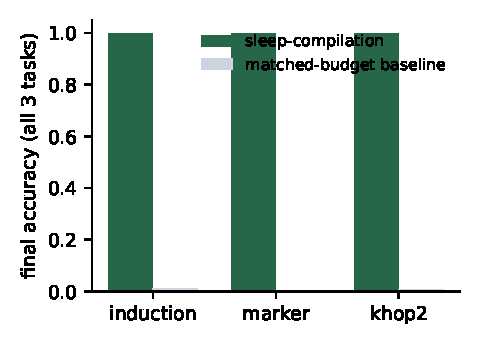
\includegraphics[width=0.8\linewidth]{figures/curriculum.pdf}
\caption{Zero forgetting by compilation: three-task curriculum, no replay. The contrast is
budget-matched on the first two tasks. \tagp{empirical}}
\label{fig:curriculum}
\end{figure}

\section{Real Text}
\label{sec:text}

On wikitext at 256-token context, no prior variant of this architecture had beaten a trained
bigram lookup (0.148); the assembled learner reaches \textbf{0.199} online, and the
package-expressible \emph{certified core} alone (counts $+$ proved rules, abstention counted
wrong) reaches $0.191$ --- a certifiability tax of only $0.008$. Certification also produced the
sharpest diagnosis: the learned soft head is a weak approximation ($0.022$ hard-alone) of the
program it approximates ($0.614$ on the copy subset), so the certified program was
\emph{installed} --- and in the autonomous version the sleep judge discovers and installs the
rules itself, rejecting every candidate for two cycles before admitting induction at $L{=}1$ and
$L{=}3$, ending at $0.201$ with a copy-subset rule marginal of $+0.058$ vs.\ $+0.042$ for the
hand-built variant: \emph{the machine's rule choices beat ours} \tagp{empirical}.

\section{Imitating Transformers: the Race and the Scaling Law}
\label{sec:race}

\textbf{Teachers.} Pythia decisions on the same 80k windows. (An inherited reference number ---
``final-residual decode $0.189$'' --- proved to be a linear-probe artifact; the true decode is
$0.244$ at 12-token context, and teacher gold at $L{=}256$ runs $0.244\!\to\!0.485$ across the
ladder.) Teachers are \emph{more} rule-shaped than their corpus: the copy-pattern incidence of
pythia-70m's decisions is 29\% (gold: 20\%), the judge admits all three induction depths within
three sleeps, and rule value roughly $2.5\times$'s.

\textbf{The race.} Against an independent decompiler (gated $n$-gram mining over the same corpus
region, its shipped thresholds), on the same held-out windows, same teacher:

\begin{table}[h]
\caption{Learning vs.\ analysis routes, teacher-decision agreement (abstain $=$ miss).
\tagp{empirical}}
\label{tab:race}
\small
\begin{tabular}{lccc}
\toprule
arm & cover & agree & when-fired \\
\midrule
analysis (shipped, det$\ge$1.0) & 3.6\% & 0.025 & \textbf{0.688} \\
analysis (det$\ge$0.5) & 16.9\% & 0.089 & 0.523 \\
\textbf{learning: certified core} & 99.2\% & \textbf{0.276} & 0.279 \\
learning: full student & 100\% & 0.352 & 0.352 \\
\bottomrule
\end{tabular}
\end{table}

Each route wins its own objective (total imitation vs.\ bounded-expert precision). The deepest
result is \textbf{convergence}: on the 480 bigram contexts both routes rule on, they give the same
answer \textbf{476/480 (99.2\%)} --- corpus statistics mined by a decompiler and counts
accumulated by a learner, agreeing on what the teacher is.

\textbf{The scaling law.} Fixing the student and rule library and walking the teacher ladder
(Fig.~\ref{fig:scaling}): the certified core declines gently ($0.285 \to 0.230$, near-flat above
410M) --- \emph{no collapse across 200$\times$ parameters} --- while crystallization
(core/student) \emph{rises} to a $\sim$85\% plateau. Structure splits as circuit theory predicts:
$n$-gram-shapedness of teacher decisions decays fastest ($-24\%$), the induction bump is durable
($-16\%$). Control: adjacent teachers agree $0.51 \to 0.75$ up the ladder, and the certified
core's $0.230$ agreement with pythia-2.8b is $\sim$65\% of what a \emph{full 14M-parameter
transformer} achieves against the same teacher ($0.351$). Confounds are stated: fixed student
capacity and library mean falling curves bound \emph{this student}, not certifiability --- the
flat core and rising ratio are the strong results because they appear despite those bounds
\tagp{empirical, this ladder and these windows}.

\begin{figure}[h]
\centering
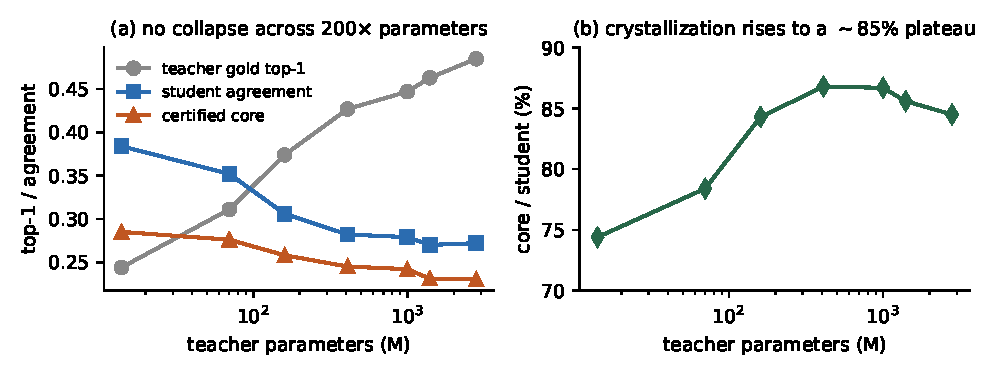
\includegraphics[width=\linewidth]{figures/scaling.pdf}
\caption{The certifiability scaling law across the Pythia ladder. \tagp{empirical}}
\label{fig:scaling}
\end{figure}

\section{The Rule-Library $\times$ Dataset Matrix}
\label{sec:library}

We extended the library as far as a held-out judge would admit --- induction $L{=}1..5$, $k$-gram
suffix tables, skip-bigrams, gapped \emph{gate} frames (grid-enumerated, then \emph{mined}:
anchored $\{$offset$:$token$\}$ frames and 2-anchor conjunctions discovered from the student's
residual errors, interaction-scored at anchor granularity), relation rules, online tiers --- and
across datasets (wikitext; a wikitext-103 control; C/C++ source).

Three portable lessons emerged, each caught by the machinery:
(1) \textbf{overlapping-window statistics inflate support} (stride-1 windows repeat each corpus
pair $\sim$21$\times$; a naive support gate is no gate);
(2) \textbf{high-variance candidates re-admit under validation noise whenever offered} ---
pre-gate strength must scale with table variance, and families need their own thresholds;
(3) \textbf{the fixed-priority cover was the dominant bottleneck}: new families mostly
\emph{displaced} the count tier rather than adding to it.

Fixing (3) is the headline. \textbf{Support-weighted arbitration} --- every applicable rule fires;
the answer with the highest confidence wins, where table rules use per-key Laplace-shrunk
determinism $c/(t+\alpha)$ (fields the serving manifest already ships) and scalar kinds use
held-out fired-accuracy (one new field) --- is worth more than every rule family combined
(Fig.~\ref{fig:library}): $+0.032$--$0.047$ on natural text and a \emph{doubling} on code
($0.31 \to 0.60$), where the certified core then \emph{exceeds the soft student that discovered
the rules} ($0.604 > 0.569$) \tagp{empirical}. The arbitration guarantee is also now formal: with per-cell
\emph{calibrated} confidences, argmax arbitration dominates every policy --- every fixed tier
priority included --- and an $\varepsilon$-miscalibrated arbiter is within
$2\varepsilon\cdot(\text{total weight})$ of optimal (\code{argmax\_policy\_optimal},
\code{miscalibration\_bound}; kernel-checked) \tagp{proved, over the stated finite cells}.
Mined frames are then the only family that still
adds on natural text ($+0.005$--$0.007$, arc bests), admitting a handful of frames per sleep on
diffuse wiki errors and dozens on structured code errors --- and correctly declining where
recovery is thin.

\begin{figure}[h]
\centering
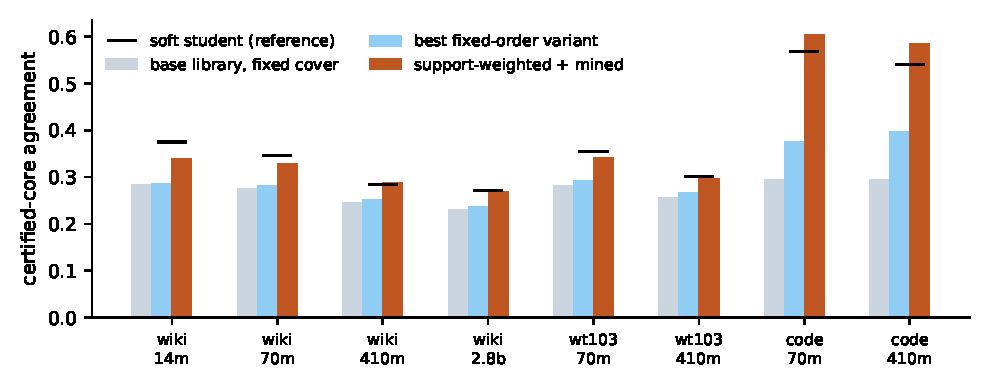
\includegraphics[width=\linewidth]{figures/library.pdf}
\caption{Certified-core agreement across the dataset matrix: base library, best fixed-order
variant, and support-weighted arbitration with mined frames; the soft student as reference. On
code the certified core exceeds its own student. \tagp{empirical}}
\label{fig:library}
\end{figure}

\section{Deployment}
\label{sec:deploy}

The rules live in an expert-package schema served host-side (no model at inference). We
contributed the \code{relation} kind (eq-guard $+$ copy; the learned repetition rule is
$eq{=}[[1,2]], copy{=}1$, admitted at $0.944$ fired-accuracy) and the \code{confidence} field to
the schema and both runtimes (reference Python and a C++ spoke), with verified parity --- the
parity test itself caught a routing bug. The spoke serves an OpenAI-compatible endpoint whose
cover miss is an explicit abstention, and a federating hub routes \emph{by} that abstention: a
wiki query fires the wiki expert, a code query the code expert, and never-seen-token gibberish is
\emph{refused in code}. Every answer cites the count evidence or the sleep cycle that admitted its
rule. Two deployment lessons: word-level relevance gates never overlap subword citations (BPE
splits identifiers), and doubled-token ``gibberish'' \emph{legitimately} fires the repetition rule
--- repeated-token continuation is real next-token behavior.

\section{Confounds and Limitations}
\label{sec:confounds}

Named throughout and collected here: fixed student capacity and hand-seeded (though
data-selected) rule families bound the student, not certifiability; top-$V$ class truncation;
5\,MB corpus slices with stride-1 window overlap; possible teacher memorization of wiki text (the
Pile); single seeds; teacher decisions at fp16 above 410M; the code corpus is one project; the
scaling ladder stops at 2.8B (VRAM). Certification is over \emph{stated domains} --- the proved
tag never travels past its test set. Wake-SGD-only multi-hop learning remains open (sleep-Adam is
the design's answer; the purist question stands), and the runtimes' shipped cover is still
fixed-priority --- the arbitration gains are measured in the learner and proposed to the schema,
not yet realized in serving. Calibration, finally, is a \emph{formal} requirement rather than an
observation: C10's dominance premise is per-cell confidence calibration on the evaluation
measure, and its $2\varepsilon$ envelope is exactly what low-support confidence inflation --- the
val-variance episodes --- consumes; the support pre-gates and per-family judge thresholds are the
mechanisms that keep $\varepsilon$ small.

\section{Conclusion}

The loop runs end to end with no transformer in the inference path: \emph{learn (SGD, wake/sleep)
$\to$ harden (anneal to discreteness) $\to$ certify (Souffl\'e, proved on stated domains) $\to$
extract (weights to Datalog, mechanically) $\to$ install (preempting structure) $\to$ package
(a schema with provenance and confidence) $\to$ serve and federate (citations, honest abstention)}.
What we take to be the durable findings: consolidation can be compilation, and certified structure
is the strongest anti-forgetting mechanism we tested; a transformer's behavior is more
crystallizable than its training text, and more so the more structured the domain; the certified
fraction does not collapse with teacher scale; arbitration beats rule supply; and two independent
routes to the same artifact agree where they overlap --- which is the closest thing a
decompilation program has to external validation.

\bibliographystyle{ACM-Reference-Format}
\bibliography{refs}

\end{document}
